\chapter{Review of Global Illumination and MC Ray Tracing}
%\chapter{Theoretical Foundations}
\label{sec:theory}

This chapter reviews important concepts about  global illumination techniques such as \textit{Ray Tracing}, followed by 
a description of 
%important explanations about 
the techniques implemented by the renderers used in our work (MC Ray Tracing). We do not delve too deep in the implementations of the techniques discussed in this chapter - we provide a general understanding of the process in order to better situate the reader.

\section{Global Illumination Algorithms}

Global illumination algorithms try to synthesize realistic pictures by
%have as their goal add more realistic lighting to 3D scenes, 
taking into account both direct and indirect illumination, at the expense of a higher computational cost when compared to local illumination techniques. 
%the Light Transport around the scene, and not only the light coming directly from the light source. 
%Images rendered using these algorithms are more photorealistic than images rendered using direct illumination algorithms at the expense of a higher computational cost. 

{\it Light transport} models the interaction between light and the surface in the scene, 
%using the principle that 
where some fraction of the light incident to a surface is reflected back to the environment. Modeling this reflection requires its spectral and directional distributions, which differ depending on the material properties of the surface. Earlier algorithms modeled these materials as ideal diffuse (Lambertian surfaces) and ideal specular (mirrors) for simplicity.

Starting at a light source (L), a light ray may bounce several times at specular (S) and diffuse (D) surfaces before reaching the eye (E). These interactions can be represented using regular expressions such as L(S|D)*E. Rendering algorithms can be caracterized by the kinds of paths they support.

Local illumination models, such as the Phong lighting model, 
%Gouraud Shading or Phong Shading, 
have the light hit the scene once before reaching the eye (LDE or LSE). Algorithms that have a good representation of specular reflection, such as Ray Tracing~\cite{Whitted:1980}, perform at most one bounce on diffuse surfaces and can perform any number of bounces on specular surfaces (LDS*E or LS*E).

\section{Ray Tracing}

\textit{Ray Tracing} \cite{Whitted:1980} is a global illumination algorithm that handles multiple inter-reflections among shiny surfaces, producing 
high-quality results for shiny surfaces. In Ray Tracing, we trace rays from the eye through each pixel of the image, searching for the closest intersected object along each ray. When an intersecting surface is found, the algorithm shoots a shadow ray to determine whether this surface is hidden from the light source and locally evaluates an illumination function. The incoming ray is then either reflected or refracted (in other words, \textit{bounced}), repeating the process until 
%the original ray reaches 
a certain amount of bounces is achieved, the contributions of subsequent hits become negligible, or the ray does not intersect any other object in the scene. This process is illustrated in Figure \ref{fig:raytracing}.

\begin{figure}[h]
  \centering
  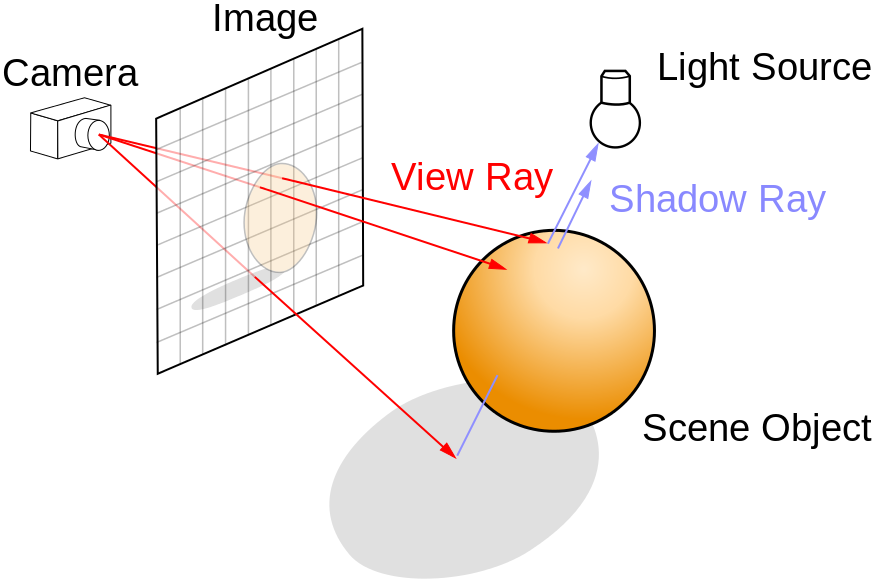
\includegraphics[width=0.45\textwidth,height=\textheight,keepaspectratio]{images/3_theoretical_foundations/raytracing.png}
  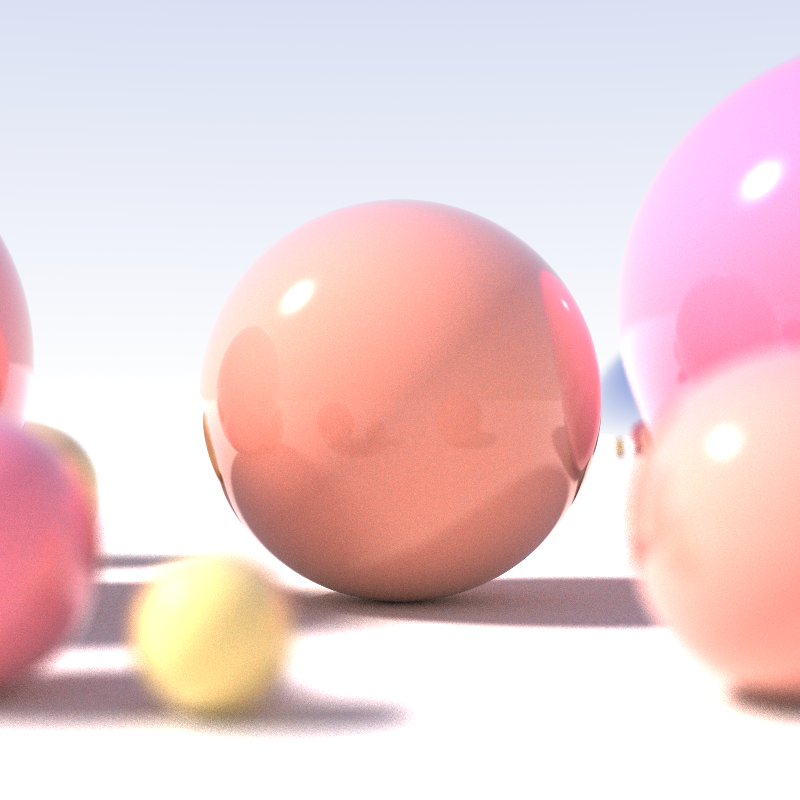
\includegraphics[width=0.45\textwidth,height=\textheight,keepaspectratio]{images/3_theoretical_foundations/raytracingexample.png}
  \caption{Visual illustration of the Ray Tracing algorithm (left) and an example of a scene rendered with the algorithm (right), extracted from \cite{wiki:raytracing}}
  \label{fig:raytracing}
\end{figure}

% While it may seem strange to send rays away from the camera - which is the opposite of how photographs are generated -, it is more cost-efficient as most light rays that incide on the scene do not reach the camera. Computing light paths is a strenuous task, and cutting back on this task load shortens the rendering time considerably.

Because a Lambertian surface reflects rays in all directions, there is a very-high computational cost associated with calculating reflections in diffuse surfaces. In order to reduce this cost, Ray Tracing algorithm approximates the actual diffuse reflection, thus not representing it with as much realism as a specular surface.

True realism can only be achieved when an algorithm approximates the \textit{Rendering Equation} \cite{Kajiya:1986} - which describes the full light transport.
%every physical effect of light flow. 
This method will be further discussed in our next section. 

\section{The Rendering Equation}

An important concept for global illumination algorithms is that of \textit{radiance}, which describes how much power arrives at (or leaves from) a certain point on a surface per unit solid angle and per unit projected area. Radiance can be thought of as the number of photons arriving per time at a small area from a given direction, and it describes the intensity of light at a given point in space in a given direction. Radiance remains constant along the light rays passing through empty space, and when computed, it captures the appearance of objects in the scene.

Another important concept is that of the \textit{Bidirectional Reflection Distribution Function} (BRDF), a function that describes the local illumination model of a given material. The BRDF can be perceived as a constant of proportionality between the amount of incident light and the reflected light along a direction. 

The BRDF has some crucial properties that aid in modeling a realistic global illumination model. It is, in general, anisotropic - which means that adding light from several incident directions in a given point has no influence on the amount of light that is reflected from it. Also, we can calculate the total amount of light reflected by a surface in a specific direction as an hemispherical integral over all possible incident directions, as seen in Figure \ref{fig:brdf}.

\begin{figure}[h]
  \centering
  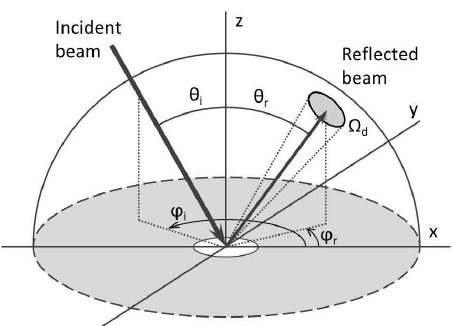
\includegraphics[width=0.5\textwidth,height=\textheight,keepaspectratio]{images/3_theoretical_foundations/brdf.png}
  \caption{Example of how BRDF describes a local illumination model for a surface, extracted from \cite{brdf}}
  \label{fig:brdf}
\end{figure}


These concepts and properties were used in the \textit{Rendering Equation} \cite{Kajiya:1986}, which models the global light transport in a scene. Modeling global illumination means that one would need to consider the light path across the entire scene, not only one interaction - which was the main problem with techniques such as Ray Tracing. 

The Rendering Equation is described as:

$$L_o (x \rightarrow \omega) = L_e (x \rightarrow \omega) + \int_{\Omega} f_r (x, s \rightarrow \omega) L_i (x \leftarrow s) V(x, x') G(x, x') ds $$

It can be interpreted as: the radiance ($L_o$) leaving a particular point ($x$) in a given direction ($\omega$) is composed of the radiance emitted ($L_e$) by this point and the reflected radiance ($L_i$) in every possible direction considering the object's BRDF ($f_r$), the visibility ($V$) and the geometry ($G$) associated. 

The Rendering Equation cannot be directly evaluated, as radiance (L) is present in both sides of the equation; it is impractical to solve with traditional quadrature methods. However, this equation \textit{can} be evaluated by \textit{Monte Carlo Integration}, the technique used in \textit{Monte Carlo Ray Tracing}.

\subsection{Monte Carlo Ray Tracing}

Monte Carlo Integration (MCI) is a technique that uses statistics principles to estimate complicated integrals. It assumes that if a $x$ is a random variable, then $f(x)$ is also a random variable that can be characterized by its probability distribution. We can approximate $f(x)$ with n random samples along $f(x)$'s probability distribution $p(x)$. The MC estimator of an arbitrary function $g(x)$ can be expressed as:

$$ \int g(x)dx \approx \frac{1}{n} \sum_{i = 1}^{n} \frac{g(X_i)}{p(X_i)}$$

The convergence rate for MCI is $O(\frac{1}{\sqrt{n}})$ regardless of the smoothness of the integrand. The technique requires only sampling and point evaluation and can be used to solve a vast array of problems. It does, however, have a high variance that can, in the case of MC rendering, appear as noise. In order to reduce the variance naturally produce by this method, one must greatly increase the number of samples.

The concept of \textit{Importance Sampling} was created to reduce this high variance, exploiting the fact that the MC estimator converges faster if the points are sampled from a distribution $p(x)$ that is similar to $f(x)$. This process is illustrated in Figure \ref{fig:importance}

\begin{figure}[h]
  \centering
  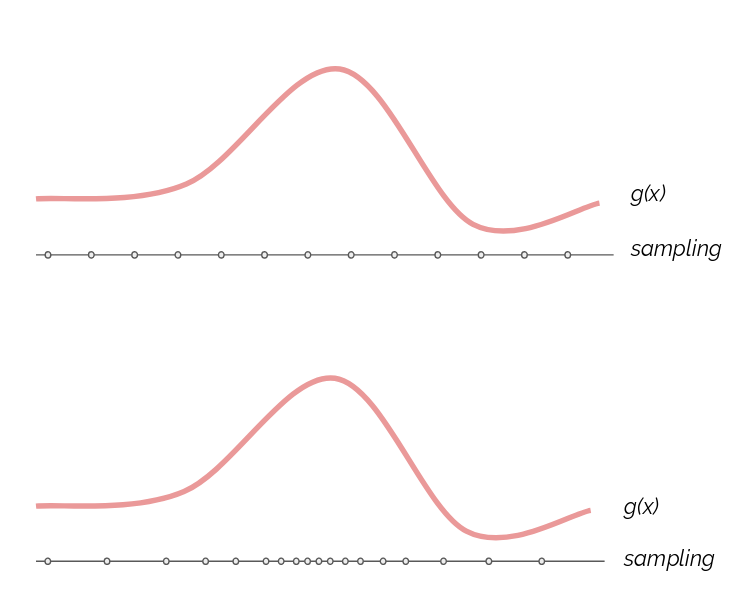
\includegraphics[width=0.5\textwidth,height=\textheight,keepaspectratio]{images/3_theoretical_foundations/importances.png}
  \caption{Illustration of how uniform sampling (top) and how importance sampling (bottom) sample $g(x)$}
  \label{fig:importance}
\end{figure}

MC Ray Tracing uses MCI to approximate the Rendering Equation, estimating the radiance for each point and produce photorealistic images. It is able to naturally reproduce very complicated effects such as motion blur (sampling over time) and depth-of-field (sampling through a lens). However, MC Ray Tracing has a very high computational cost - even using Importance Sampling, the number of samples required to render a large scene is in the order of thousands per pixel. Generating these images can take up to hours depending on the complexity of the scene. 

Notwithstanding, MC Ray Tracing is currently the only practical solution for simulating global illumination effects in complex environments. It is implemented in virtually every modern physically-based renderer, featuring several other algorithms using MCI, such as Photon Mapping and Metropolis Light Transport.